\let\negmedspace\undefined
\let\negthickspace\undefined
\documentclass[journal,12pt,onecolumn]{IEEEtran}
\usepackage{cite}
\usepackage{amsmath,amssymb,amsfonts,amsthm}
\usepackage{algorithmic}
\usepackage{graphicx}
\graphicspath{{./figs/}}
\usepackage{textcomp}
\usepackage{xcolor}
\usepackage{txfonts}
\usepackage{listings}
\usepackage{enumitem}
\usepackage{mathtools}
\usepackage{gensymb}
\usepackage{comment}
\usepackage{caption}
\usepackage[breaklinks=true]{hyperref}
\usepackage{tkz-euclide} 
\usepackage{gvv}                                        
\usepackage[latin1]{inputenc}     
\usepackage{xparse}
\usepackage{color}                                            
\usepackage{array}
\usepackage{longtable}                                       
\usepackage{calc}                                             
\usepackage{multirow}
\usepackage{multicol}
\usepackage{hhline}                                           
\usepackage{ifthen}                                           
\usepackage{lscape}
\usepackage{tabularx}
\usepackage{array}
\usepackage{float}
\newtheorem{theorem}{Theorem}[section]
\newtheorem{problem}{Problem}
\newtheorem{proposition}{Proposition}[section]
\newtheorem{lemma}{Lemma}[section]
\newtheorem{corollary}[theorem]{Corollary}
\newtheorem{example}{Example}[section]
\newtheorem{definition}[problem]{Definition}
\theoremstyle{remark}
\newtheorem{rem}{Remark}

\begin{document}

\title{5.9.2}
\author{Revanth Siva Kumar D EE25BTECH11048}
\maketitle

\textbf{Question :} The present age of a father is three years more than three times the age of his son. Three years hence the father's age will be 10 years more than twice the age of the son. Determine their present ages.

\textbf{Solution :} 

Let 
\[
x = \text{son's present age}, \quad y = \text{father's present age}.
\]

From the problem statement:

1. \textbf{Father's present age is three years more than three times son's age}:
\[
y = 3x + 3 \quad \Rightarrow \quad -3x + y = 3
\]

2. \textbf{Three years hence, father's age will be 10 years more than twice son's age}:
\[
y + 3 = 2(x+3) + 10 \quad \Rightarrow \quad -2x + y = 13
\]

\begin{table}[h!] \centering \begin{tabular}{|c|c|}
\hline
\textbf{Name} & \textbf{Value} \\ \hline
$\vec{A}$ & $\myvec{2 & 1 \\0 & 3}$ \\ \hline
\end{tabular}
 \caption*{Table : Equations} \label{5.9.2} \end{table}

Writing in matrix form:

\begin{align}
\myvec{-3 & 1\\-2 & 1}\myvec{x\\y} &= \myvec{3\\13}
\end{align}

Forming the augmented matrix:

\begin{align}
\myaugvec{2}{-3 & 1 & 3\\-2 & 1 & 13}
\end{align}

Using Gaussian elimination:

\begin{align}
\myaugvec{2}{-3 & 1 & 3\\-2 & 1 & 13} 
\xleftrightarrow{\;R_2 \to R_2 - \frac{2}{3}R_1\;}
\myaugvec{2}{-3 & 1 & 3\\0 & \frac{1}{3} & 11}
\end{align}

Back substitution gives:

\begin{align}
\frac{y}{3} &= 11 \\
y &= 33\\
-3x + y &= 3 \;\Rightarrow\; -3x + 33 = 3 \;\Rightarrow\; x = 10
\end{align}

\begin{align}
\myvec{x\\y} &= \myvec{10\\33}
\end{align}

Therefore, the present ages are:

\begin{align*}
\text{Son's age } &= 10 \text{ years} \\
\text{Father's age } &= 33 \text{ years}
\end{align*}
\pagebreak
\begin{figure}[H]
    \centering
    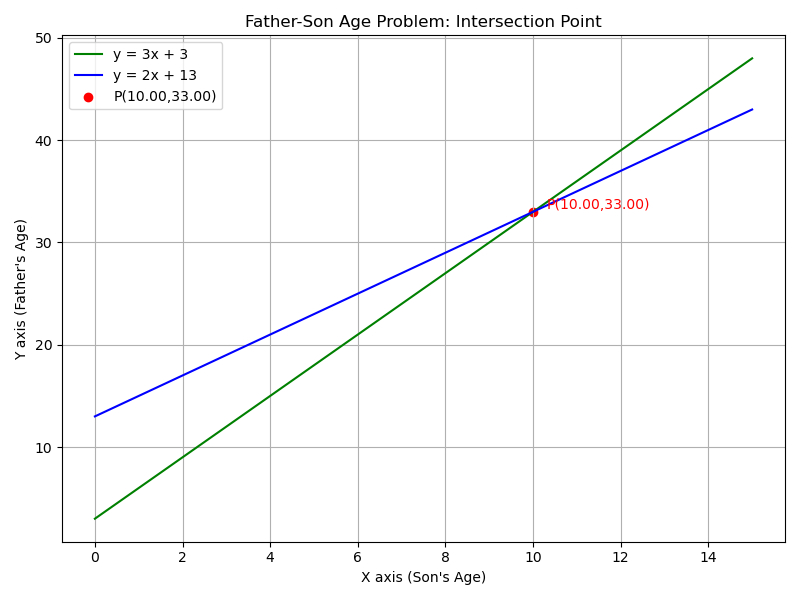
\includegraphics[width=0.7\columnwidth]{figs/Figure_1.png}
    \caption{PLOT}
    \label{fig:placeholder}
\end{figure}
\end{document}
